% -*- TeX-master: "../Qualificacao.tex" -*-
%!TEX root = ../Qualificacao.tex

\chapter{Randomized Controller Structure Selection}\label{cap:CCS}
\vspace{-1cm}

% Frase citação inicial {{{1
% \begin{flushright}
% \begin{minipage}{0.7\linewidth}
%     \emph{``\dots''}
% \end{minipage}
% \end{flushright}
%
% \begin{flushright}
% Cicrano
% \end{flushright}
%
%\vspace{1cm}

% Intro CAP {{{2

Neste capítulo, são apresentadas propostas para projeto de controladores DDC no que diz respeito à escolha de estrutura do controlador. A metodologia utilizada, assim como os resultados preliminares obtidos nas primeiras etapas da pesquisa são apresentados.

Nesta pesquisa, o foco tem sido dado ao estudo e desenvolvimento de técnicas de seleção de estruturas para o modelo de controladores realimentados em procedimento de projeto DDC\@.
A intenção é, no âmbito de controle de sistemas não lineares, adaptar técnicas de seleção de estruturas conhecidas na área de identificação de sistemas para lidar com o caso de controle, onde neste caso, o sistema a ser identificado, passa a ser o controlador. Para atingir estes objetivos optou-se pelo uso de modelos polinomiais para representação dos controladores, inicialmente com estruturas NARX\@. Esta escolha é conveniente devido à característica de flexibilidade estrutural e a capacidade desses modelos em descrever sistemas não lineares~\citep{pearson1999,martins2013}.
% \begin{figure}[htpb]
% \centering
% \missingfigure{Pretendo colocar por aqui um diagramas (deve ser blocos) para ajudar.}
% % \includegraphics[width=0.8\textwidth]{}
% \caption{}
% \label{fig:Diagrama representativo}
% \end{figure}
%

As mentioned in Chapter~\ref{cap:cap2}, one of the main steps in the system identification procedure from data is the step of choosing the model structure. Works that aim to help on this task have been proposed, as is the case of the works developed by~\cite{baldacchino2012,baldacchino2013} and \cite{falsone2014,falsone2015}.
\todo{Colocar aqui também sobre o ERR, etc.} 

in which a random approach is used in order to select the best candidates among the possible regressors in the formation of the model to be identified.

% As mentioned in Chapter~\ref{cap:cap2}, one of the main steps in the procedure of model system identification from data is the model selection step.  Studies that aim to deal with this task have been proposed, as is the case of studies developed by~\cite{falsone2014, falsone2015} in which a random approach, named RaMSS, is used in order to select the best candidates to compose a final model structure, among a class of possible regressors.

% \todo{Confirmar se o RaMSS original só é aplicável a NARX mesmo na sua forma original. Se for, falar aqui.}
Mais recentemente,~\cite{retesNARMAXModelIdentification2019} estenderam a estratégia RaMSS para escolha de estruturas de modelos NARMAX, que levam em conta o efeito de ruídos nos sinais no intuito de reduzir a polarização nas estimativas paramétricas. 
\todo{Colocar aqui mais referências neste sentido. Seleção de estruturas.} 

No âmbito de projeto de controladores baseado em dados, mais especificamente pelo método VRFT, em que o os parâmetros do controlador são ajustados por técnicas de identificação convencionais como OLS, ILS, IV, dentre outras, o mesmo problema de escolha de estrutura do modelo ocorre, com a diferença que agora o modelo representa o controlador, e não mais o processo. Portanto, analogias devem poder serem feitas em relação ao uso do método RaMSS no intuito de estendê-lo para fins de identificação da estrutura mais adequada para o controlador.

Neste sentido, o presente trabalho tem se voltado ao estudo das possibilidades e consequências do uso dessas tecnologias para escolha da estrutura do controlador que se mostre mais adequada para fins de controle. 

\todo[inline]{Pretendo colocar um paragrafo aqui comentando o que será apresentado no restante do capítulo.} 


\section{Methodology}\label{sec:CSS_metod} \todo{Talvez colocar o Título como: ``The RaCSS Methodology''"?}
\todo[inline]{A terminar... Vou mexer no início e fim desta seção ainda, enquanto estiver traduzindo.} 

% Como metodologia para atingir este objetivo, listam-se as etapas a seguir, que por sua vez são detalhadas nas seções subsequentes:
Visando atingir o objetivo final de se utilizar uma estratégia para estrutura e identificação paramétrica de controladores a partir de uma abordagem DDC, pretende-se neste trabalho, fazer uso das duas metodologias abordadas em capítulos anteriores: o VRFT, para sintonia de parâmetros do controlador e o RaMSS, para seleção da melhor estrutura do controlador. A partir de do estudo e adaptações de trabalhos anteriores \citep{retesNARMAXModelIdentification2019}, tem-se desenvolvido um algoritmo capaz de unir as duas estratégias com o objetivo de auxiliar tanto na seleção de estruturas, quando na sintodia de controladores não-lieares (ou lineares). O algoritmo tem servido de  framework para estudo e validação da abordagem proposta, a partir de simuações numéricas. Neste sentido, parte dos esforços da pesquisa tem se voltado para a implemetação numérica deste framework. Em uma primeira etapa, foi analisado o comportamento do algoritmo na identificação de modelos de processos, a partir do algoritmo RaMSS, como proposto originalmente. Alguns dos resultados de validação desta etapa são apresentados no Capítulo \ref{cap:cap2}, sob a forma do Exemplo \ref{ex:varHeater}.

Uma vez validado o funcionamento do algorítmo, o método VRFT, discutido no Capítulo \ref{cap:VRFT} é acrescentado ao processo, de forma que o desempenho do RaMSS em selecionar estruturas para um controlador possa ser avaliado na prática.
Nesta etapa, o algoritmo RamSS, utilizado no Capítulo \ref{cap:cap2} é ligeiramente modificado para lidar com a esimação paramétrica via VRFT, para primeiros testes de projeto de controladores. Neste cenário se espera alguns primeiros resultados, sem maiores compromissos com bons desempenhos, mas de são de grande valia para análise e comparação das modificações propostas. Alguns destes resuldados são apresentados pelos exemplos da seção \ref{sec:prel_results} a seguir, mais especificamente no exemplo \ref{ex:51}.

Como abordado no Capítulo \ref{cap:VRFT}, sob certas condições, o controlador pode ser identificados por procedimentos tradicionais de identificação de sistemas pelo método VRFT. Caso as condições necessárias não sejam satisfeitas (vide a Assumption \ref{ass:machedControl} -- matched control) um filtro pode ser projetado de forma que a minimização do índice de custo relativo aos sinais de entrada e saída do controlador, dado por $J_{VR}(\bm{\theta})$ resulte também na minimização do índice de custo $J_{MR}(\bm{\theta})$ relativo ao erro de rastreamento de um modelo de referência. Esta relação é garantida pelo filtro desde que a estrutura do modelo não seja muito ``distante'' da estrutura ideal, i.e. desde que não seja muito subparametrizada.

Uma proposta é utilizar o procedimento RaMSS para tentar identificar a estrutura ideal para o controlador, ou pelo menos uma estrutura próxima que gere bons resultados ao se utilizar o procedimento VRFT. A identificação desta estrutura é feita a partir de dados colhidos sob a abordagem VRFT. Na tentativa de validar a proposta simulações são feitas em diferentes cenários. 
Em um primeiro cenário o procedimento RaMSS é aplicado a um processo linear onde seu modelo e o modelo do controlador ideal são previamente conhecidos. O intuito aqui é analisar o comportamento do procedimento na seleção de regressores candidatos a um eventual controlador. Uma análise ao estilo Monte Carlo é aplicada ao processo em 2 casos: no primeiro, o procedimento é realizado sem influência de ruídos nos dados utilizados; no segundo, ruídos são acrescentados aos dados no intuito de simulação de um ambiente mais realista. O Exemplo \ref{ex:sis2aord} analisa estes casos.

O procedimento RaMSS foi originalmente proposto para lidar com identificação de processos, e não controladores.
A atualização do vetor de probabilidades para inclusão dos regressores (RIPs) é feita baseando-se em índices de desempenho visando avaliar a qualidade de predição do modelo. 
Esta predição é feita sobre dados de treinamento, utilizando uma versão exponencial do MSSE, e possivelmente, no intuito de aumentar a robustez, sobre dados de validação (free run simulation) por meio de uma versão exponencial do MSSE.
No entanto, para fins de controle, tais índices podem não ser os melhores.
Principalmente o índice baseado no MSSE, que exige maior custo computacional sob a proposta de promover melhoras na robustez do modelo identificado. O efeito é uma melhor predição do sinal de saída do do modelo identificado, mesmo quando excitado com sinais diferentes daqueles usados na identificação. 
Apesar de carecer de mais estudos, a princípio este índice não parece trazer muitos benefícios quando utilizado para fins MSS do controlador, uma vez que o intuito final, no projeto de um controlador, é fazer com que o sinal de saída do processo (e não do controlador), tenha um comportamento desejado. 

Neste sentido, propõe-se adaptações ao método RaMSS original visando objetivos mais adequados a MSS de controladores. Uma modificação estudada, é a substituição da versão exponencial do MSSE, dada por $J_s= e^{-K\cdot MSSE}$, por uma que leve em conta o rastreamento do sistema em malha fechada, um dos principais objetivos do controlador. Este novo índice é definido como
\begin{equation}
  J_r=e^{-K\cdot MSTE},
  \label{eq:}
\end{equation}
onde $MSTE$, é o erro médio quadrático de rastreamento, definido como 
\begin{equation}
  MSTE = \frac{1}{N}\sum_{k=1}^{N} (y_{rm}(k)-y(k))^2.
  \label{eq:}
\end{equation}

Uma vez que a escolha de estrutura é feita pelo método RaMSS modificado, incorporando elementos da estratégia VRFT, e que o intutito é a seleção de estrutura e parâmetros para controladores, batiza-se, aqui, esta estratégia de \textit{Randomized Controler Structure Selection}, ou RaCSS.

Resultados preliminares do uso deste índice são apresentados nesta qualificação. Os Exemplos \ref{ex:52} e \ref{ex:53} apresentam alguns destes resultados e uma análise geral é feita no Capítulo \ref{cap:Concl}. \todo{colocar a referencia correta aqui.} 

Ressalta-se que os resultados apresentados são preliminares e conclusões concretas ainda não puderam ser apresentadas. 
\todo{batizar o método de RaCSS.} 
No Capítulo \ref{cap:Concl}, propostas para continuidade do trabalho, como inclusão de informações auxiliares ao procedimento, objetivando incorporar características previamente desejadas ou conhecidas para o controlador, assim como possivelmente o uso de estratégias de aprendizado por reforço, no intuito de reduzir o custo computacional devido ao uso de informações da malha fechada do controlador são apresentadas.

Por fim, discussões a respeito de estabilidade, convergência, polarização e robustez são apresentadas, ainda não em um contexto de garantias, mas como conjecturas de passos que pretende-se aprofundar na sequência da presente pesquisa.

\section{Preliminary Results}\label{sec:prel_results}

\begin{exmp}[Second order Linear System -- continued.]\label{ex:sis2aord}

  Consider the 2nd-order linear system describe in Example \ref{exm:31}: 
  \begin{equation}
    \label{eq:sis2aord}
    y_k = a_1y_{k-1} + a_2y_{k-2} + b_1u_{k-1} + b_2u_{k-2}.
  \end{equation}
  % onde, para $i = 1,\ 2$, os termos $a_i$, $b_i$ $\in \R$, representam parâmetros constantes; $u_{k-i}$ e $y_{k-i}$ $\in \R$, os sinais de entrada e saída, respectivamente; e $k$ o índice temporal.
  According to the VRFT strategy (Chapter ~\ref{cap:VRFT}), one must first define a class of allowable controllers $\mathscr{C}$, containing the desired controller structure, and define a reference model that expresses the desired close loop system's behavior.

  In this example, we want to analyze the use of the RAmSS algorithm directly, without modifications, in order to find the best structure for a controller designed from the VRFT strategy.
  In order to examine the behavior of the RaMSS Algorithm in finding the best set of regressors, we proceed as follows.

  A feasible reference model is defined, that is, with a relative degree equal to or greater than that of the process. For simplicity, a 1st order model with the same relative degree of the process is chosen, as Example \ref{exm:31}, given by the transfer function
  \begin{equation}
    T_d(z) = \frac{1-A}{z-A},
    \label{eq:mr_sis2aord}
  \end{equation}
  The parameter adopted here is the same as Exemple \ref{exm:31}, i.e. $A = -T_s/\tau_d = 0.8187$. 
  The ideal controller, represented by an ARX model, will be given by the structure composed of the regressors presented in \eqref{eq:exp31_uk}, represented here by
  \begin{equation}
    \label{eq:exp51_contIdeal}
    u_k = \theta_0e_{k} + \theta_1e_{k-1} + \theta_2e_{k-2} + \theta_3u_{k-1} + \theta_4u_{k-2},
  \end{equation}
  and will have the parameters shown in \eqref{eq:exp31_ideal_parameters}, described here as
  \begin{equation}
    \vtheta^\star= \begin{bmatrix} \theta^\star_0 & \theta^\star_1 & \theta^\star_2 & \theta^\star_3 & \theta^\star_4 \end{bmatrix}^T =  \begin{bmatrix} 0.181 & 0.308 &  0.145 &  0.19 & 0.81 \end{bmatrix}^T.
  \label{eq:ex51_ideal_parameters}
\end{equation}
Using the RaMSS algorithm, as discussed in the section ~\ref{sec:ramss}, the procedure is performed for 2 cases:
\begin{description}
  \item[case A] the universe set $\mathscr{M}$ is taken as all possible 3rd degree non linear models formed by the monomials up to 4 delays for input $\tilde{e}_k$ (virtual error) and output $\tilde{u}_k$ (virtual process input) collected data. No noise is considered in this case.
  \item[case B] the same case as case A, but now with a noise given by a gaussian distribution, i.e. $\nu \sim \mathcal{N}(\mu,\sigma)$, where $\mu=0$ is the mean, and $\sigma= 0.1$ is the standard deviation.
\end{description}
The simulation parameters for the 2 cases are shown in the table ~\ref{tab:exp51_param}.


\begin{table}[htpb]
  \centering
  \caption{Parameters for simulating the RaMSS algorithm of the example ~\ref{ex:sis2aord}}\label{tab:exp51_param}
  \begin{tabular}{c|c|c|c|c|c|c|c}
    Caso & $o$ & $n_e$ & $n_m$ & $N_p$ & $N_i$ & $K_J$ & $\gamma$ \\
    \hline
    1 & $ 1 $ & $7$ & $4$ & $100$ & $100$ & $1$ & $0.1$ \\
    2 & $ 2 $ & $7$ & $4$ & $100$ & $100$ & $1$ & $0.1$
  \end{tabular}
\end{table}
\todo[inline]{MEXER NESTA TABELA AINDA! Valores estão errados. Já os modifiquei. Definir parâmetros, etc. Colocar os mais essenciais por aqui e os menos, no appendice. }

O procedimento RaMSS é aplicado a um conjunto de dados de 700 amostras, obtido via procedimento VRFT, em que o filtro do VRFT é considerado unitário, i.e os dados não são filtrados. O mesmo conjunto de dados é aplicado para os 2 casos. A cada iteração escolhe-se aleatoriamente, por uma processo de Bernoulli, 100 modelos candidatos a serem analisados. Os RIPs são atualizados em, no máximo, 100 iterações, ou até todos convergirem para uma margem acima de 0.9 ou abaixo de 0.1, i.e. adota-se o seguinte critério de parada:
\begin{align}
  \textbf{if } \left[iter<iter_{\max}\right] \textbf{ or } \left[\Delta_S < \frac{1}{2} \left(1-\min_{\forall \mu \in \bm{\mu}_k}{ \left| 2\mu -1 \right| }\right)\right] \textbf{ then} \text{, STOP the procedure.}
\label{eq:}
\end{align}
onde $\Delta_S = 0.1$ é a margem de convergência, $iter$ é o número da iteração e $iter_{\max} = 100$ é o máximo de iterações permitido. 

       % <- (1-min(abs(2*mu.vec.df[,iter]-1)))/2

Applying the procedure in both cases, the following controllers are obtained, for a specific realization:
\begin{align*}
  u_1(k) &= 0.193{u}_1(k-1) + 0.805{u}_1(k-2) + 0.001{u}_1(k-3) \\
         &+ 0.181{e}_1(k) + 0.307{e}_1(k-1) + 0.1441 \\
  u_2(k) &= 0.751{u}_2(k-1) + 0.241{u}_2(k-2) -0.33{u}_2(k-3) + 0.322{u}_2(k-4) \\
         &+ 0.174{e}_2(k) + 0.197{e}_2(k-1) + 0.048{e}_2(k-2) + 0.049{e}_2(k-3) + 0.0591
  % \label{eq:contEstsis2aord}
\end{align*}
where the index subscribed to the variables represent the respective cases.

The table ~\ref{tab:exp51_param} sumarizes the simulation parameters used in \ref{alg:RaMSS}, for the 2 cases.
\begin{table}[htpb]
  \centering
  \caption{Parameters for simulating the RaMSS algorithm of the example ~\ref{ex:sis2aord}}\label{tab:exp51_param}
  \begin{tabular}{c|c|c|c|c|c|c|c|c}
    Case & $o$ & $n_{\tilde{e}}$ & $n_{\tilde{u}}$ & $ N_p$ & $ iter_{\max} $ & $K$ & $\gamma_0$  & $\nu$\\
    \hline
    A & $ 3 $ & $4$ & $4$ & $100$ & $100$ & $1$ & $2$ & $0$ \\
    B & $ 3 $ & $4$ & $4$ & $100$ & $100$ & $1$ & $2$ & $\mathcal{N}(\mu,\sigma)$
  \end{tabular}
\end{table}

onde  $o$ é o grau máximo permitido para os regressores, $n_{\tilde{e}}$ é o máximo de atraso para o sinal de erro virtual $\tilde{e}(k)$, $n_{\tilde{u}}$ é o máximo atraso para o sinal de entrada da planta amostrado,  $ N_p$ é o número de modelos escolhidos a cada atualização dos RIPs, $ iter_{\max} $ é o número máximo de iterações permitidas, $\Delta_S$ é o trashold para convergência dos RIPs, $K$ é o ganho para os índices de desempenho apresentados em \ref{eq:Js}, $\gamma_0$ é o ganho inicial de \ref{eq:gamma} e  $\nu$ o ruído adicionado a saída\\
\todo[inline]{MEXER NESTA TABELA AINDA! Valores estão errados. Já os modifiquei. Definir parâmetros, etc. Colocar os mais essenciais por aqui e os menos, no appendice. }

The evolution of RIPs during a typical execution is shown in \ref{fig:ex51_RIPevol_2cases}.
\begin{figure}[H]
  \centering
  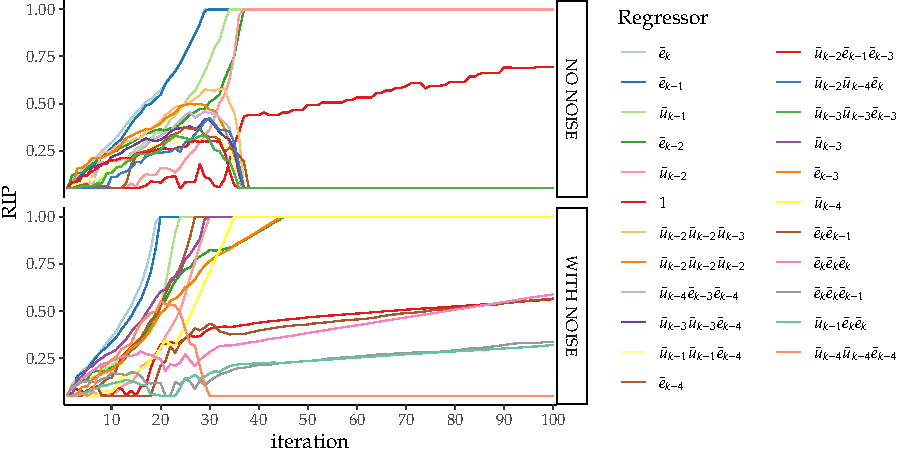
\includegraphics[width=\textwidth]{Figs/Cap5/ex51_rips_evol_2cases.tex.pdf}
  \caption{Typical evolution of RIPs for choosing regressors for case 1 and 2.}
  \label{fig:ex51_RIPevol_2cases}
\end{figure}


A figura~\ref{fig:Figs-RespostaSist2aordNARX-png} mostra a resposta temporal para os 2 casos.

\begin{figure}[H]
  \sbox0{\blackdottedline} \sbox1{\bluesolidline} \sbox2{\reddashedline} \sbox3{\blackdashdotline} 
  \centering
  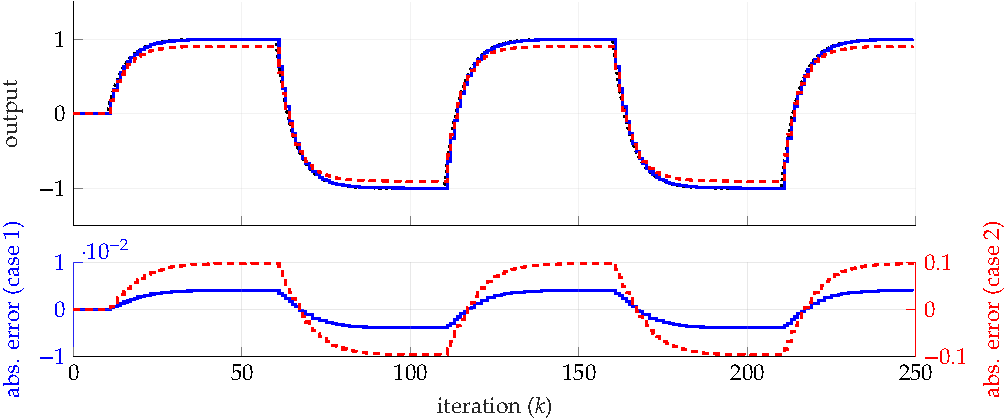
\includegraphics[width=1\textwidth]{./Figs/Cap5/ex51_resp_temporal_mf_editado.tex.pdf}
  % % This file was created by matlab2tikz.
%
%The latest updates can be retrieved from
%  http://www.mathworks.com/matlabcentral/fileexchange/22022-matlab2tikz-matlab2tikz
%where you can also make suggestions and rate matlab2tikz.
%
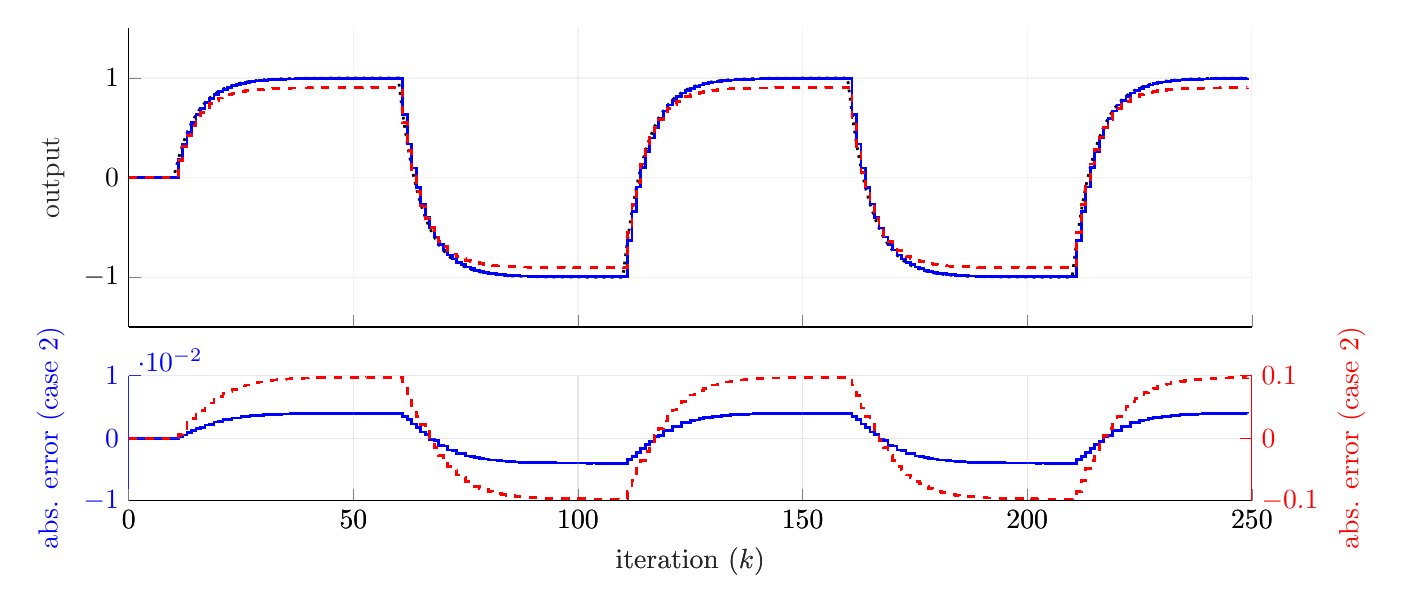
\begin{tikzpicture}

\begin{axis}[%
width=14.264cm,
height=3.794cm,
at={(0cm,2.206cm)},
scale only axis,
xmin=0,
xmax=250,
xtick={0,50,100,150,200,250},
xticklabels={{},{},{},{},{},{}},
ymin=-1.5,
ymax=1.5,
ylabel style={font=\color{white!15!black}},
ylabel={output},
axis background/.style={fill=white},
axis x line*=bottom,
axis y line*=left,
xmajorgrids,
ymajorgrids,
grid style={opacity=0.2}
]
\addplot [color=black, dotted, line width=1.0pt, forget plot]
  table[row sep=crcr]{%
0	0\\
10	0\\
11	0.181269246922028\\
12	0.329679953964359\\
13	0.45118836390597\\
14	0.550671035882772\\
15	0.632120558828547\\
16	0.69880578808781\\
17	0.753403036058387\\
18	0.798103482005331\\
19	0.834701111778401\\
20	0.8646647167634\\
21	0.88919684163767\\
22	0.909282046710587\\
23	0.925726421785669\\
24	0.939189937374778\\
25	0.950212931632137\\
26	0.959237796021625\\
27	0.966626730039678\\
28	0.972676277552694\\
30	0.981684361111263\\
32	0.987722660096921\\
34	0.991770252950971\\
37	0.995483419057393\\
41	0.997970569363702\\
47	0.999388747238868\\
60	0.999954600070225\\
61	0.637424335837267\\
62	0.340609659588267\\
63	0.0975983561783096\\
64	-0.10136247126897\\
65	-0.264257819357908\\
66	-0.397625250371675\\
67	-0.506817267601633\\
68	-0.596216130098412\\
69	-0.669409728114744\\
70	-0.729335577739135\\
71	-0.778398713730951\\
72	-0.818568212009893\\
73	-0.85145621558658\\
74	-0.878382635522144\\
75	-0.900428123593684\\
76	-0.918477442644473\\
77	-0.933254975223463\\
78	-0.945353795600482\\
79	-0.955259471919135\\
80	-0.963369553751249\\
81	-0.970009527157174\\
82	-0.975445877584235\\
84	-0.983540879531887\\
86	-0.988967121610102\\
88	-0.992604440449782\\
91	-0.995941230863423\\
95	-0.998176277468275\\
102	-0.999550275560608\\
110	-0.999909202201621\\
111	-0.637387167206128\\
112	-0.340579228486888\\
113	-0.0975734412997724\\
114	0.101382869846248\\
115	0.264274520300432\\
116	0.397638923946914\\
117	0.506828462578198\\
118	0.596225295770012\\
119	0.669417232331938\\
120	0.72934172167254\\
121	0.778403743958165\\
122	0.818572330411598\\
123	0.851459587448716\\
124	0.878385396169364\\
125	0.900430383820463\\
126	0.918479293161653\\
127	0.933256490298788\\
128	0.945355036039246\\
129	0.955260487504489\\
130	0.963370385242229\\
131	0.970010207924418\\
132	0.975446434949305\\
134	0.983541253144864\\
136	0.988967372050382\\
138	0.99260460832491\\
141	0.995941322995236\\
145	0.998176318865774\\
152	0.999550285769089\\
160	0.999909204262678\\
161	0.637387168893582\\
162	0.340579229868467\\
163	0.0975734424308996\\
164	-0.101382868920155\\
165	-0.264274519542226\\
166	-0.397638923326127\\
167	-0.506828462069933\\
168	-0.596225295353889\\
169	-0.669417231991247\\
170	-0.72934172139361\\
171	-0.778403743729797\\
172	-0.81857233022464\\
173	-0.851459587295636\\
174	-0.878385396044024\\
175	-0.900430383717861\\
176	-0.918479293077638\\
177	-0.933256490230008\\
178	-0.945355035982942\\
179	-0.955260487458389\\
180	-0.963370385204456\\
181	-0.970010207893495\\
182	-0.975446434923981\\
184	-0.983541253127925\\
186	-0.988967372039014\\
188	-0.992604608317293\\
191	-0.995941322991058\\
195	-0.998176318863898\\
202	-0.999550285768635\\
210	-0.999909204262593\\
211	-0.637387168893497\\
212	-0.34057922986841\\
213	-0.0975734424308712\\
214	0.101382868920183\\
215	0.264274519542255\\
216	0.397638923326156\\
217	0.506828462069961\\
218	0.596225295353918\\
219	0.669417231991275\\
220	0.72934172139361\\
221	0.778403743729797\\
222	0.81857233022464\\
223	0.851459587295636\\
224	0.878385396044052\\
225	0.900430383717861\\
226	0.918479293077638\\
227	0.933256490230008\\
228	0.945355035982942\\
229	0.955260487458389\\
230	0.963370385204485\\
231	0.970010207893495\\
232	0.975446434923981\\
234	0.983541253127925\\
236	0.988967372039014\\
238	0.992604608317293\\
241	0.995941322991058\\
245	0.998176318863898\\
249	0.999180567244224\\
};
\addplot[const plot, color=blue, line width=1.0pt, forget plot] table[row sep=crcr] {%
0	0\\
11	0.180977171837526\\
12	0.329172712212909\\
13	0.45031150992321\\
14	0.54950721174589\\
15	0.630603534262377\\
16	0.697071838198383\\
17	0.75129926836172\\
18	0.795887192211239\\
19	0.832113918402939\\
20	0.862042313411223\\
21	0.886239644815532\\
22	0.906320094899854\\
23	0.922499135273426\\
24	0.935950021055618\\
25	0.946791840399243\\
26	0.955778629339733\\
27	0.963064221517527\\
28	0.969052500940336\\
29	0.973959104837405\\
30	0.977943604763652\\
31	0.981248875948808\\
32	0.983902902127539\\
33	0.986123664527099\\
34	0.987898809353766\\
35	0.98938291118904\\
36	0.990577874726654\\
37	0.991563033579666\\
38	0.99237257824521\\
39	0.99302302327095\\
40	0.993573142885879\\
41	0.994002292764549\\
42	0.994375004464132\\
43	0.994660023006162\\
44	0.99491004110115\\
45	0.995101960911995\\
46	0.995267159859196\\
47	0.995398551232711\\
48	0.995506018603493\\
49	0.995597031866481\\
50	0.995666340606363\\
51	0.995729353060426\\
52	0.995774354984661\\
53	0.995817277218976\\
54	0.995847290647959\\
55	0.995875646946359\\
56	0.995896489317232\\
57	0.995914513739081\\
58	0.99592950784691\\
59	0.995940580406312\\
60	0.995951482435515\\
61	0.634003883369871\\
62	0.337620550089099\\
63	0.0953472448544233\\
64	-0.10303894571345\\
65	-0.2652285809788\\
66	-0.39816195207419\\
67	-0.506614475468581\\
68	-0.595788499822845\\
69	-0.668240060126379\\
70	-0.728095910664535\\
71	-0.776489090096334\\
72	-0.816649504165156\\
73	-0.849006521870962\\
74	-0.875907972279464\\
75	-0.897590947700024\\
76	-0.915564224598512\\
77	-0.930135072159629\\
78	-0.942111315794165\\
79	-0.951924405502382\\
80	-0.959893102619901\\
81	-0.966503635844077\\
82	-0.971811439975454\\
83	-0.976252980102885\\
84	-0.979803103504366\\
85	-0.982771300351828\\
86	-0.985161145199214\\
87	-0.987131422548657\\
88	-0.98875049439485\\
89	-0.990051322178317\\
90	-0.99115157956436\\
91	-0.992009815056377\\
92	-0.992755265095326\\
93	-0.993325252586487\\
94	-0.993825306183027\\
95	-0.994209118582432\\
96	-0.994539518302446\\
97	-0.994802294746677\\
98	-0.995017218301086\\
99	-0.995199252164724\\
100	-0.995337852432442\\
101	-0.995463889534307\\
102	-0.995553877257976\\
103	-0.995639731886712\\
104	-0.995699748235978\\
105	-0.995756465549192\\
106	-0.995798146571843\\
107	-0.995834194602935\\
108	-0.995864184425045\\
109	-0.995886325211501\\
110	-0.995908133508522\\
111	-0.633967273804899\\
112	-0.337591692291056\\
113	-0.0953226731259633\\
114	0.103058301629801\\
115	0.265244929159081\\
116	0.398175062764892\\
117	0.506625249266051\\
118	0.595797451149849\\
119	0.668247118158689\\
120	0.728102030832304\\
121	0.776493725318176\\
122	0.816653654829679\\
123	0.84900960826289\\
124	0.875910738485828\\
125	0.897593050066035\\
126	0.915566026255306\\
127	0.930136537077203\\
128	0.942112465237926\\
129	0.951925437303544\\
130	0.959893831175947\\
131	0.966504355793973\\
132	0.971811911211717\\
133	0.976253467082586\\
134	0.979803423931486\\
135	0.982771614147225\\
136	0.985161376691991\\
137	0.987131613667088\\
138	0.988750668125164\\
139	0.990051433495751\\
140	0.991151709211351\\
141	0.992009880262856\\
142	0.992755357103761\\
143	0.993325294868953\\
144	0.993825365970537\\
145	0.994209151088342\\
146	0.994539552657386\\
147	0.994802322807573\\
148	0.995017235142114\\
149	0.995199276392725\\
150	0.99533785939127\\
151	0.995463908745052\\
152	0.995553880291141\\
153	0.995639745123498\\
154	0.995699750932573\\
155	0.995756472981157\\
156	0.995798150277864\\
157	0.99583419749294\\
158	0.995864188932899\\
159	0.995886325370492\\
160	0.99590813792517\\
161	0.633967272955033\\
162	0.337591695755407\\
163	0.0953226724599574\\
164	-0.103058299551094\\
165	-0.265244929117785\\
166	-0.398175062008676\\
167	-0.506625248547522\\
168	-0.595797451309551\\
169	-0.668247117097962\\
170	-0.728102031391813\\
171	-0.776493724302242\\
172	-0.816653655361904\\
173	-0.849009607559282\\
174	-0.875910738755806\\
175	-0.89759304976053\\
176	-0.915566026223672\\
177	-0.930136537101305\\
178	-0.942112464997905\\
179	-0.951925437508748\\
180	-0.959893830868879\\
181	-0.966504356028963\\
182	-0.971811910957314\\
183	-0.976253467244817\\
184	-0.979803423791878\\
185	-0.982771614199692\\
186	-0.985161376669453\\
187	-0.987131613626559\\
188	-0.988750668181922\\
189	-0.99005143340699\\
190	-0.991151709296645\\
191	-0.992009880172304\\
192	-0.992755357175952\\
193	-0.993325294807619\\
194	-0.993825366007997\\
195	-0.994209151066315\\
196	-0.994539552658807\\
197	-0.994802322817804\\
198	-0.995017235119491\\
199	-0.995199276419669\\
200	-0.995337859360859\\
201	-0.99546390877299\\
202	-0.995553880266129\\
203	-0.995639745142142\\
204	-0.99569975091967\\
205	-0.995756472987182\\
206	-0.995798150277125\\
207	-0.995834197488733\\
208	-0.995864188940118\\
209	-0.995886325361141\\
210	-0.995908137934919\\
211	-0.633967272945597\\
212	-0.337591695763365\\
213	-0.0953226724537615\\
214	0.103058299547115\\
215	0.265244929119746\\
216	0.398175062008619\\
217	0.506625248546129\\
218	0.59579745131208\\
219	0.668247117094865\\
220	0.728102031395082\\
221	0.7764937242992\\
222	0.816653655364519\\
223	0.849009607557321\\
224	0.875910738757113\\
225	0.897593049759934\\
226	0.915566026223644\\
227	0.930136537101816\\
228	0.942112464997081\\
229	0.951925437509772\\
230	0.959893830867799\\
231	0.966504356029986\\
232	0.971811910956461\\
233	0.976253467245471\\
234	0.979803423791452\\
235	0.982771614199862\\
236	0.985161376669453\\
237	0.987131613626389\\
238	0.988750668182206\\
239	0.990051433406649\\
240	0.991151709297014\\
241	0.992009880171963\\
242	0.992755357176208\\
243	0.99332529480742\\
244	0.993825366008139\\
245	0.994209151066258\\
246	0.994539552658807\\
247	0.99480232281789\\
248	0.995017235119377\\
249	0.995199276419783\\
};
\addplot[const plot, color=red, dashed, line width=1.0pt, forget plot] table[row sep=crcr] {%
0	0\\
11	0.175057837660773\\
12	0.315108606907074\\
13	0.426588150709449\\
14	0.51956167119738\\
15	0.594286109260821\\
16	0.655135784739997\\
17	0.702527697924609\\
18	0.741838777618398\\
19	0.77225983010905\\
20	0.798373587886005\\
21	0.817964067832179\\
22	0.8350736083475\\
23	0.847611071714567\\
24	0.858723810104294\\
25	0.866922466539478\\
26	0.874060824457501\\
27	0.879513082557196\\
28	0.883999242995742\\
29	0.887673652014797\\
30	0.890462181039311\\
31	0.892949013964\\
32	0.894689964971832\\
33	0.896343978862291\\
34	0.897461842614717\\
35	0.898523537010391\\
36	0.899278919205585\\
37	0.899927562215879\\
38	0.900463534863803\\
39	0.90083967915939\\
40	0.901227428975886\\
41	0.90143979655096\\
42	0.901713732305325\\
43	0.901839323230234\\
44	0.902020253342215\\
45	0.902106347904407\\
46	0.902213540384309\\
47	0.902283235255084\\
48	0.902337553824992\\
49	0.902397723252136\\
50	0.902419819972835\\
51	0.902469326037533\\
52	0.902476441913677\\
53	0.902512513076459\\
54	0.90251623038057\\
55	0.902538032212703\\
56	0.902543914642166\\
57	0.902553458871893\\
58	0.902562340116049\\
59	0.90256361457989\\
60	0.902573698170528\\
61	0.552455445478785\\
62	0.272362786933741\\
63	0.0494007823988909\\
64	-0.136540247295017\\
65	-0.285990440390719\\
66	-0.407687067631656\\
67	-0.502470205440403\\
68	-0.581092278701334\\
69	-0.641932311178806\\
70	-0.694161189176867\\
71	-0.733339692463602\\
72	-0.767560412461251\\
73	-0.79263335075575\\
74	-0.814859956970821\\
75	-0.831256182941274\\
76	-0.845533232563184\\
77	-0.856437559375536\\
78	-0.865409538605803\\
79	-0.872758770170918\\
80	-0.878335140896809\\
81	-0.88330943754994\\
82	-0.886790649753493\\
83	-0.890099211291471\\
84	-0.892334474714488\\
85	-0.894458138169568\\
86	-0.895968736547701\\
87	-0.897266028287817\\
88	-0.898338051108368\\
89	-0.899090166389698\\
90	-0.899865869116638\\
91	-0.900290373633823\\
92	-0.900838455599256\\
93	-0.901089448591165\\
94	-0.901451449058101\\
95	-0.901623540769322\\
96	-0.901837971016619\\
97	-0.901977355190809\\
98	-0.902085960258347\\
99	-0.902206353892666\\
100	-0.9022504763999\\
101	-0.90234956258152\\
102	-0.902363722937849\\
103	-0.902435925631892\\
104	-0.902443313274432\\
105	-0.902486947330146\\
106	-0.902498697163736\\
107	-0.902517786090243\\
108	-0.902535559211117\\
109	-0.902538089185128\\
110	-0.90255827970293\\
111	-0.552437424800161\\
112	-0.272353669518367\\
113	-0.0493887280749448\\
114	0.136546275187442\\
115	0.285997795158806\\
116	0.407691694069229\\
117	0.502474143318068\\
118	0.581096134216409\\
119	0.641934087841918\\
120	0.694164336115279\\
121	0.733340374593951\\
122	0.767562741271121\\
123	0.792633684597831\\
124	0.814861425197137\\
125	0.831256561092516\\
126	0.845533945951161\\
127	0.8564380834612\\
128	0.865409719746452\\
129	0.872759366985946\\
130	0.87833504778024\\
131	0.8833099779593\\
132	0.886790497812001\\
133	0.890099595248756\\
134	0.892334392981667\\
135	0.894458332123122\\
136	0.895968764038798\\
137	0.89726606144643\\
138	0.898338162241629\\
139	0.899090103490011\\
140	0.899866010181398\\
141	0.900290283164196\\
142	0.900838576423098\\
143	0.901089379855762\\
144	0.901451521089001\\
145	0.901623515058702\\
146	0.901837990733185\\
147	0.901977369365483\\
148	0.902085942205645\\
149	0.902206390863569\\
150	0.902250442146482\\
151	0.902349602678896\\
152	0.902363691363718\\
153	0.902435954655999\\
154	0.902443295162755\\
155	0.902486959715276\\
156	0.902498694480471\\
157	0.902517783862891\\
158	0.902535567669759\\
159	0.902538078608103\\
160	0.902558292559149\\
161	0.552437412716728\\
162	0.272353680841377\\
163	0.0493887193443356\\
164	-0.136546268713317\\
165	-0.285997798625345\\
166	-0.407691692909395\\
167	-0.502474142154227\\
168	-0.581096136835015\\
169	-0.641934084084795\\
170	-0.694164340221533\\
171	-0.733340370465015\\
172	-0.767562744884572\\
173	-0.792633681658486\\
174	-0.814861427224344\\
175	-0.831256559933763\\
176	-0.845533946247315\\
177	-0.856438083843869\\
178	-0.865409718824651\\
179	-0.872759368220756\\
180	-0.878335046395961\\
181	-0.883309979307967\\
182	-0.886790496612093\\
183	-0.890099596198667\\
184	-0.892334392317451\\
185	-0.894458332484959\\
186	-0.895968763949213\\
187	-0.897266061304208\\
188	-0.898338162551482\\
189	-0.899090103073632\\
190	-0.89986601063913\\
191	-0.900290282716924\\
192	-0.900838576815858\\
193	-0.901089379544487\\
194	-0.901451521302931\\
195	-0.901623514943168\\
196	-0.901837990757684\\
197	-0.901977369415732\\
198	-0.90208594210003\\
199	-0.902206391002636\\
200	-0.90225044199417\\
201	-0.902349602826376\\
202	-0.902363691234569\\
203	-0.902435954757436\\
204	-0.902443295093491\\
205	-0.902486959751769\\
206	-0.902498694473763\\
207	-0.902517783844985\\
208	-0.902535567705542\\
209	-0.902538078561548\\
210	-0.902558292609712\\
211	-0.552437412668013\\
212	-0.272353680883754\\
213	-0.0493887193112243\\
214	0.13654626869095\\
215	0.285997798636885\\
216	0.40769169290769\\
217	0.502474142147918\\
218	0.581096136847151\\
219	0.64193408406922\\
220	0.694164340238331\\
221	0.733340370448957\\
222	0.76756274489847\\
223	0.792633681647686\\
224	0.814861427231563\\
225	0.831256559930125\\
226	0.845533946247713\\
227	0.856438083846086\\
228	0.865409718820558\\
229	0.872759368225985\\
230	0.87833504639039\\
231	0.883309979313253\\
232	0.886790496607517\\
233	0.890099596202163\\
234	0.892334392315121\\
235	0.894458332486096\\
236	0.895968763949128\\
237	0.897266061303441\\
238	0.898338162552875\\
239	0.899090103071899\\
240	0.899866010640977\\
241	0.90029028271519\\
242	0.900838576817335\\
243	0.90108937954335\\
244	0.901451521303699\\
245	0.901623514942827\\
246	0.901837990757713\\
247	0.901977369416016\\
248	0.902085942099575\\
249	0.902206391003205\\
};
\end{axis}

\begin{axis}[%
width=14.264cm,
height=1.588cm,
at={(0cm,0cm)},
scale only axis,
xmin=0,
xmax=250,
xtick={  0,  50, 100, 150, 200, 250},
xlabel style={font=\color{white!15!black}},
xlabel={iteration ($k$)},
every outer y axis line/.append style={blue},
every y tick label/.append style={font=\color{blue}},
every y tick/.append style={blue},
ymin=-0.01,
ymax=0.01,
ytick={-0.01,    0,  0.01},
ylabel style={font=\color{blue}},
ylabel={abs. error (case 2)},
axis background/.style={fill=white},
axis x line*=bottom,
axis y line*=left,
xmajorgrids,
ymajorgrids,
grid style={opacity=0.2}
]
\addplot[const plot, color=blue, line width=1.0pt, forget plot] table[row sep=crcr] {%
0	0\\
1	0\\
2	0\\
3	0\\
4	0\\
5	0\\
6	0\\
7	0\\
8	0\\
9	0\\
10	0\\
11	0.000292075084480176\\
12	0.000507241751442511\\
13	0.000876853982768211\\
14	0.00116382413687421\\
15	0.00151702456619074\\
16	0.00173394988941156\\
17	0.00210376769667719\\
18	0.00221628979410016\\
19	0.00258719337547819\\
20	0.00262240335216601\\
21	0.00295719682212836\\
22	0.00296195181074288\\
23	0.00322728651224391\\
24	0.00323991631917342\\
25	0.00342109123288703\\
26	0.00345916668188717\\
27	0.00356250852214923\\
28	0.00362377661237734\\
29	0.00367012330641792\\
30	0.00374075634761539\\
31	0.00375554723070715\\
32	0.0038197579694017\\
33	0.00382449972826293\\
34	0.00387144359722236\\
35	0.00387914181186799\\
36	0.00390556085257976\\
37	0.003920385477724\\
38	0.00392955803829997\\
39	0.00394942198368098\\
40	0.00394810493746622\\
41	0.00396827659916044\\
42	0.00396343826270495\\
43	0.00397960895628502\\
44	0.00397618375101072\\
45	0.00398615712244876\\
46	0.00398625433243327\\
47	0.00399019600617267\\
48	0.00399352996306945\\
49	0.00399323315453592\\
50	0.00399819676572899\\
51	0.00399599336960055\\
52	0.00400077769115237\\
53	0.00399861698736281\\
54	0.00400197627695031\\
55	0.00400094324955269\\
56	0.00400247128091957\\
57	0.00400276219535611\\
58	0.00400276341660322\\
59	0.00400396799425162\\
60	0.00400311763472017\\
61	0.00342045246740397\\
62	0.00298910949916176\\
63	0.00225111132390626\\
64	0.00167647444448767\\
65	0.000970761620900262\\
66	0.00053670170253789\\
67	-0.000202792133058294\\
68	-0.000427630275575797\\
69	-0.00116966798834894\\
70	-0.00123966707460521\\
71	-0.00190962363459402\\
72	-0.0019187078447348\\
73	-0.00244969371561099\\
74	-0.00247466324267154\\
75	-0.00283717589365973\\
76	-0.00291321804596179\\
77	-0.00311990306384202\\
78	-0.00324247980633918\\
79	-0.00333506641676307\\
80	-0.00347645113133588\\
81	-0.00350589131308976\\
82	-0.00363443760877347\\
83	-0.00364380476048398\\
84	-0.00373777602751957\\
85	-0.00375311155233304\\
86	-0.00380597641089231\\
87	-0.0038356206185729\\
88	-0.00385394605493539\\
89	-0.00389370578169757\\
90	-0.0038910286174958\\
91	-0.00393141580705081\\
92	-0.00392169579289658\\
93	-0.00395407309902984\\
94	-0.00394719408658994\\
95	-0.00396715888583332\\
96	-0.00396734397573517\\
97	-0.00397522748190737\\
98	-0.00398190155247902\\
99	-0.00398129647926482\\
100	-0.00399123754172281\\
101	-0.00398681579500204\\
102	-0.0039963983026271\\
103	-0.00399206488434289\\
104	-0.00399879245710966\\
105	-0.00399672044542354\\
106	-0.00399977921166095\\
107	-0.00400036102161183\\
108	-0.00400036117686398\\
109	-0.00400277410712702\\
110	-0.00400106869311345\\
111	-0.00341989340122295\\
112	-0.00298753619584657\\
113	-0.00225076817381159\\
114	-0.00167543178356248\\
115	-0.000970408858629701\\
116	-0.00053613881796849\\
117	0.000203213312159445\\
118	0.000427844620166873\\
119	0.0011701141732714\\
120	0.00123969084024012\\
121	0.00191001863999063\\
122	0.00191867558193748\\
123	0.00244997918583401\\
124	0.00247465768353172\\
125	0.00283733375442097\\
126	0.00291326690633198\\
127	0.00311995322157321\\
128	0.00324257080133794\\
129	0.0033350502009688\\
130	0.00347655406626723\\
131	0.00350585213043086\\
132	0.00363452373757811\\
133	0.00364377411269301\\
134	0.00373782921340127\\
135	0.00375310364534343\\
136	0.00380599535839243\\
137	0.00383563454330016\\
138	0.00385394019975016\\
139	0.00389373190879105\\
140	0.00389101150056026\\
141	0.00393144273239565\\
142	0.00392167921562592\\
143	0.00395409257437607\\
144	0.00394718486209822\\
145	0.00396716777743467\\
146	0.00396734351420325\\
147	0.00397522717058285\\
148	0.003981907430891\\
149	0.00398129085234122\\
150	0.00399124581218158\\
151	0.00398680905295301\\
152	0.00399640547796387\\
153	0.00399206000556518\\
154	0.00399879660345326\\
155	0.00399671861602235\\
156	0.00399978009260493\\
157	0.00400036188710118\\
158	0.00400035974375212\\
159	0.00400277646552949\\
160	0.00400106633752628\\
161	0.00341989593855241\\
162	0.00298753411306452\\
163	0.00225076997095258\\
164	0.0016754306309507\\
165	0.000970409575570597\\
166	0.000536138682531273\\
167	-0.000203213522417256\\
168	-0.000427844044339598\\
169	-0.00117011489330998\\
170	-0.0012396900017928\\
171	-0.00191001942753999\\
172	-0.00191867486272546\\
173	-0.0024499797363432\\
174	-0.00247465728822305\\
175	-0.002837333957323\\
176	-0.00291326685396387\\
177	-0.00311995312869495\\
178	-0.00324257098502245\\
179	-0.00333504994965905\\
180	-0.00347655433559468\\
181	-0.00350585186453212\\
182	-0.00363452396668873\\
183	-0.00364377392974446\\
184	-0.0037378293360445\\
185	-0.00375310357901482\\
186	-0.00380599536957138\\
187	-0.00383563457451486\\
188	-0.00385394013537876\\
189	-0.00389373199132259\\
190	-0.00389101141014303\\
191	-0.00393144281876945\\
192	-0.00392167914002972\\
193	-0.00395409263289803\\
194	-0.00394718482234657\\
195	-0.00396716779758555\\
196	-0.00396734351124772\\
197	-0.00397522715906962\\
198	-0.00398190745249094\\
199	-0.00398129082454735\\
200	-0.00399124584192367\\
201	-0.00398680902443249\\
202	-0.00399640550249958\\
203	-0.00399205998653973\\
204	-0.00399879661606162\\
205	-0.00399671860972017\\
206	-0.00399978009315893\\
207	-0.00400036189114261\\
208	-0.00400035973638824\\
209	-0.00400277647477565\\
210	-0.00400106632766373\\
211	-0.00341989594789505\\
212	-0.00298753410504804\\
213	-0.00225076997708706\\
214	-0.00167543062691854\\
215	-0.000970409577503994\\
216	-0.000536138682459331\\
217	0.00020321352385122\\
218	0.000427844041851144\\
219	0.00117011489639962\\
220	0.0012396899985363\\
221	0.00191001943060864\\
222	0.00191867486011654\\
223	0.00244997973832595\\
224	0.00247465728694085\\
225	0.00283733395791852\\
226	0.00291326685397897\\
227	0.00311995312819424\\
228	0.00324257098586322\\
229	0.0033350499486311\\
230	0.0034765543366706\\
231	0.00350585186352603\\
232	0.00363452396753938\\
233	0.00364377392910298\\
234	0.00373782933645517\\
235	0.00375310357882996\\
236	0.00380599536955673\\
237	0.00383563457468727\\
238	0.00385394013509677\\
239	0.00389373199166376\\
240	0.00389101140978809\\
241	0.00393144281909896\\
242	0.00392167913975283\\
243	0.00395409263310453\\
244	0.00394718482221668\\
245	0.00396716779764061\\
246	0.00396734351125749\\
247	0.00397522715900855\\
248	0.00398190745258664\\
249	0.00398129082443366\\
};
\end{axis}

\begin{axis}[%
width=14.264cm,
height=1.588cm,
at={(0cm,0cm)},
scale only axis,
xmin=0,
xmax=250,
xtick={  0,  50, 100, 150, 200, 250},
xlabel style={font=\color{white!15!black}},
xlabel={iteration ($k$)},
every outer y axis line/.append style={red},
every y tick label/.append style={font=\color{red}},
every y tick/.append style={red},
ymin=-0.1,
ymax=0.1,
ytick={-0.1,    0,  0.1},
ylabel style={font=\color{red}},
ylabel={abs. error (case 2)},
axis background/.style={fill=none},
axis x line*=bottom,
axis y line*=right,
xmajorgrids,
ymajorgrids,
grid style={opacity=0.2}
]
\addplot[const plot, color=red, dashed, line width=1.0pt, forget plot] table[row sep=crcr] {%
0	0\\
11	0.00621140926125463\\
12	0.0145713470572844\\
13	0.0246002131965213\\
14	0.0311093646853919\\
15	0.0378344495677254\\
16	0.0436700033477848\\
17	0.0508753381337783\\
18	0.0562647043869333\\
19	0.0624412816693507\\
20	0.0662911288773955\\
21	0.071232773805491\\
22	0.0742084383630868\\
23	0.0781153500711014\\
24	0.0804661272704834\\
25	0.0832904650926594\\
26	0.085176971564124\\
27	0.0871136474824823\\
28	0.0886770345569801\\
29	0.0899555761290571\\
30	0.0912221800719522\\
31	0.0920554092155328\\
32	0.093032695125089\\
33	0.093604185393076\\
34	0.0943084103362537\\
35	0.0947385159905423\\
36	0.0952045163736557\\
37	0.0955558568414858\\
38	0.0958386014197004\\
39	0.0961327660952236\\
40	0.0962938188474425\\
41	0.0965307728127414\\
42	0.0966247104215086\\
43	0.0968003087322131\\
44	0.096865971509942\\
45	0.0969817701300428\\
46	0.0970398738073186\\
47	0.0971055119837843\\
48	0.0971619947415832\\
49	0.0971925417688908\\
50	0.0972447173992634\\
51	0.097256020392507\\
52	0.0972986907621305\\
53	0.0973033811298762\\
54	0.0973330365443417\\
55	0.0973385579832211\\
56	0.0973550459559931\\
57	0.0973638170625293\\
58	0.0973699311474547\\
59	0.0973809338206593\\
60	0.0973809018996974\\
61	0.084968890358482\\
62	0.0682468726545267\\
63	0.0481975737794471\\
64	0.0351777760260461\\
65	0.021732621032811\\
66	0.0100618172600093\\
67	-0.00434706216123004\\
68	-0.0151238513971066\\
69	-0.0274774169359375\\
70	-0.0351743885622682\\
71	-0.045059021267349\\
72	-0.0510077995486142\\
73	-0.0588228648308018\\
74	-0.0635226785513225\\
75	-0.0691719406524101\\
76	-0.0729442100812605\\
77	-0.0768174158479269\\
78	-0.0799442569946791\\
79	-0.0825007017482164\\
80	-0.0850344128544407\\
81	-0.0867000896072341\\
82	-0.088655227830742\\
83	-0.0897975735719001\\
84	-0.0912064048173988\\
85	-0.0920662737345879\\
86	-0.0929983850624012\\
87	-0.0937010148794286\\
88	-0.0942663893414135\\
89	-0.094854861570326\\
90	-0.0951767390652094\\
91	-0.0956508572296002\\
92	-0.095838505288981\\
93	-0.0961898770943606\\
94	-0.0963210512115324\\
95	-0.0965527366989534\\
96	-0.0966688912615723\\
97	-0.0968001670377703\\
98	-0.0969131595952319\\
99	-0.0969741947513114\\
100	-0.0970786135742685\\
101	-0.097101142747789\\
102	-0.0971865526227589\\
103	-0.0971958711391494\\
104	-0.0972552274186569\\
105	-0.0972662386644743\\
106	-0.0972992286197893\\
107	-0.0973167695343307\\
108	-0.097328986390778\\
109	-0.097351010133508\\
110	-0.0973509224986913\\
111	-0.0849497424059678\\
112	-0.0682255589685212\\
113	-0.0481847132248276\\
114	-0.0351634053411942\\
115	-0.021723274858374\\
116	-0.0100527701223143\\
117	0.00435431926013052\\
118	0.0151291615536024\\
119	0.0274831444900485\\
120	0.0351773855572617\\
121	0.0450633693642146\\
122	0.0510095891404774\\
123	0.0588259028508844\\
124	0.0635239709722271\\
125	0.0691738227279473\\
126	0.0729453472104922\\
127	0.0768184068375888\\
128	0.0799453162927932\\
129	0.0825011205185433\\
130	0.0850353374619601\\
131	0.0867002299650892\\
132	0.0886559371373039\\
133	0.0897976459465326\\
134	0.0912068601632257\\
135	0.0920663856694546\\
136	0.0929986080115839\\
137	0.0937011867639512\\
138	0.0942664460832816\\
139	0.0948550619145578\\
140	0.0951767105305237\\
141	0.09565103983104\\
142	0.0958384598962994\\
143	0.0961900075875803\\
144	0.0963210297436206\\
145	0.0965528038070715\\
146	0.0966689054384062\\
147	0.0968001806126608\\
148	0.0969132003673678\\
149	0.096974176381508\\
150	0.0970786630570046\\
151	0.0971011151191021\\
152	0.0971865944054002\\
153	0.0971958504730708\\
154	0.0972552523732872\\
155	0.0972662318818891\\
156	0.0972992358900058\\
157	0.0973167755171573\\
158	0.097328981006882\\
159	0.0973510232279011\\
160	0.0973509117035292\\
161	0.0849497561768544\\
162	0.0682255490270904\\
163	0.0481847230865924\\
164	0.0351633997931629\\
165	0.0217232790831474\\
166	0.0100527695832682\\
167	-0.00435431991570567\\
168	-0.0151291585189028\\
169	-0.0274831479064517\\
170	-0.0351773811720477\\
171	-0.0450633732647816\\
172	-0.0510095853400685\\
173	-0.0588259056371498\\
174	-0.0635239688197089\\
175	-0.069173823784098\\
176	-0.0729453468303234\\
177	-0.0768184063861383\\
178	-0.0799453171582911\\
179	-0.0825011192376337\\
180	-0.0850353388085239\\
181	-0.0867002285855278\\
182	-0.0886559383119163\\
183	-0.0897976449759028\\
184	-0.0912068608104448\\
185	-0.092066385293748\\
186	-0.0929986080898004\\
187	-0.0937011868968511\\
188	-0.0942664457658111\\
189	-0.0948550623246831\\
190	-0.0951767100676761\\
191	-0.0956510402741344\\
192	-0.0958384595001291\\
193	-0.0961900078960127\\
194	-0.0963210295274166\\
195	-0.0965528039207015\\
196	-0.0966689054123719\\
197	-0.0968001805611323\\
198	-0.0969132004719313\\
199	-0.0969741762415879\\
200	-0.0970786632085776\\
201	-0.0971011149710534\\
202	-0.0971865945340653\\
203	-0.0971958503712358\\
204	-0.0972552524422383\\
205	-0.0972662318451398\\
206	-0.0972992358965143\\
207	-0.0973167755348925\\
208	-0.097328980970957\\
209	-0.0973510232743706\\
210	-0.0973509116528817\\
211	-0.084949756225484\\
212	-0.0682255489846568\\
213	-0.0481847231196468\\
214	-0.0351633997707665\\
215	-0.0217232790946298\\
216	-0.010052769581506\\
217	0.00435431992204371\\
218	0.0151291585067952\\
219	0.0274831479220552\\
220	0.0351773811553073\\
221	0.0450633732808399\\
222	0.0510095853261703\\
223	0.0588259056479501\\
224	0.0635239688124898\\
225	0.069173823787736\\
226	0.0729453468299255\\
227	0.0768184063839215\\
228	0.0799453171623838\\
229	0.0825011192324325\\
230	0.0850353388140945\\
231	0.0867002285802414\\
232	0.0886559383164638\\
233	0.0897976449724069\\
234	0.0912068608127754\\
235	0.0920663852926111\\
236	0.0929986080898857\\
237	0.0937011868976469\\
238	0.0942664457644184\\
239	0.0948550623264168\\
240	0.0951767100658287\\
241	0.0956510402758681\\
242	0.0958384594986228\\
243	0.096190007897178\\
244	0.0963210295266492\\
245	0.096552803921071\\
246	0.0966689054123435\\
247	0.0968001805608765\\
248	0.0969132004724145\\
249	0.0969741762410194\\
};
\end{axis}
\end{tikzpicture}%

  \caption{Resposta do sistema em malha fechada (gráfico superior) e respectivos erros absolutos (gráfico inferior) utilizando os controladores identificados no caso A (\usebox1) e no caso B (\usebox2). Os sinais de referência (\usebox3) e de reposta do modelo de de referência (\usebox0) são mostrados no gráfico superior.}
  \label{fig:Figs-RespostaSist2aordNARX-png}
\end{figure}

\todo[inline]{Ainda em construção, por enquanto só coloquei alguns dos gráficos que irei utilizar. Comparações, com tabelas comparando resultados do RaCSS com o ERR também serão ainda colocados. Logicamente, com devidas análises.}

\end{exmp}

\begin{exmp}[RaCSS aplicado a um sistema linear de 2$^a$ ordem] \label{ex:52}

  \todo[inline]{    
    Neste exemplo aplico o ``RaCSS'' ao mesmo sistema de 2a ordem do exemplo anterior, mas agora usando informação do erro de rastreamento no cálculo dos RIPs.

    Por enquanto estão somente os gráficos, ainda falta análise e algumas tabelas comparativas com ERR.
  }

  Evolução dos RIPs para um caso típico:

  \begin{figure}[H]
    \centering
    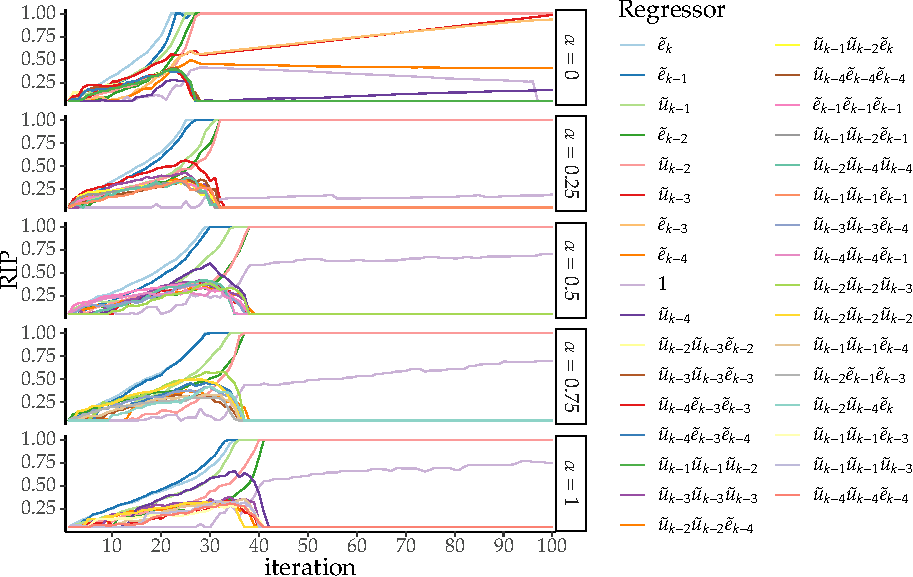
\includegraphics{Figs/Cap5/ex51_rips_evol_SR.tex.pdf}
    \caption{Evolução dos RIPs para diferentes valores da parâmetro $\alpha$ considerando dados sem ruído. ({\color{red} Caption ainda será mudada.})}
    \label{fig:exp51_ev_rips_a1}
  \end{figure}

  \begin{figure}[H]
    \centering
    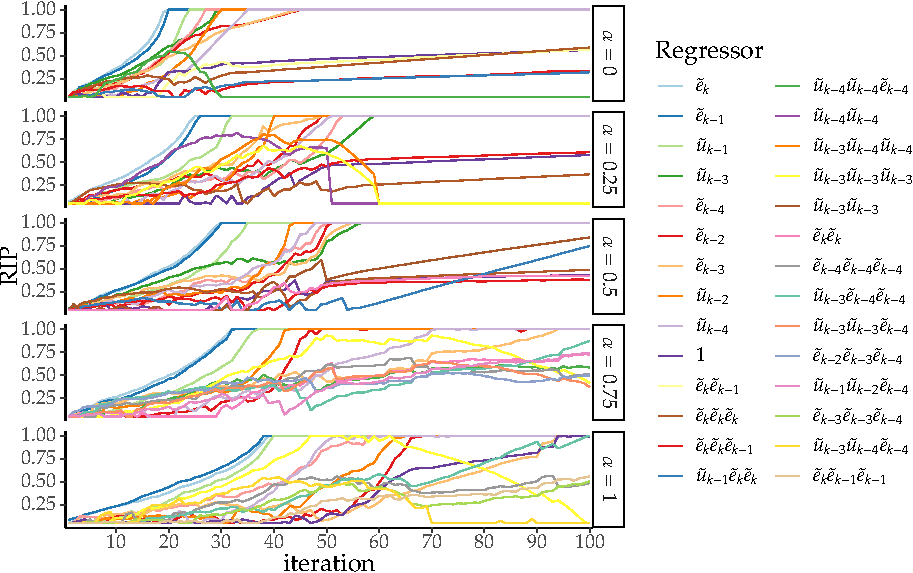
\includegraphics{Figs/Cap5/ex51_rips_evol_CR.tex.pdf}
    \caption{Evolução dos RIPs para diferentes valores da parâmetro $\alpha$ considerando dados COM ruído. ({\color{red} Caption ainda será mudada.})}
    \label{fig:exp51_ev_rips_a1}
  \end{figure}



  Convergência dos regressores para 100 simulações para cada parâmetro $\alpha$ diferente:

  \begin{figure}[H]
    \centering
    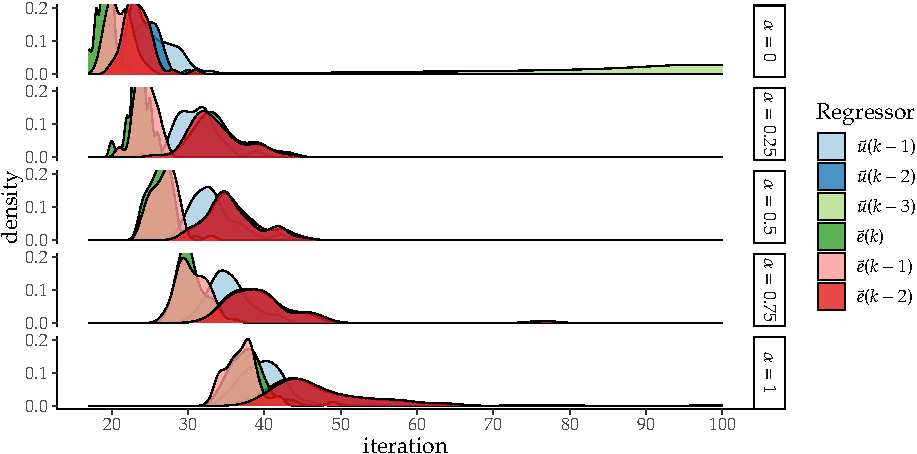
\includegraphics{Figs/Cap5/ex51_iter_con_SEM_ruido.tex.pdf}
    \caption{Densidades de probabilidades para os regressores escolhidos para diferentes valores de $\alpha$, caso sem ruído.({\color{red} Caption ainda será mudada.})}
    \label{fig:exp51_itercon_ruido}
  \end{figure}

  \begin{figure}[H]
    \centering
    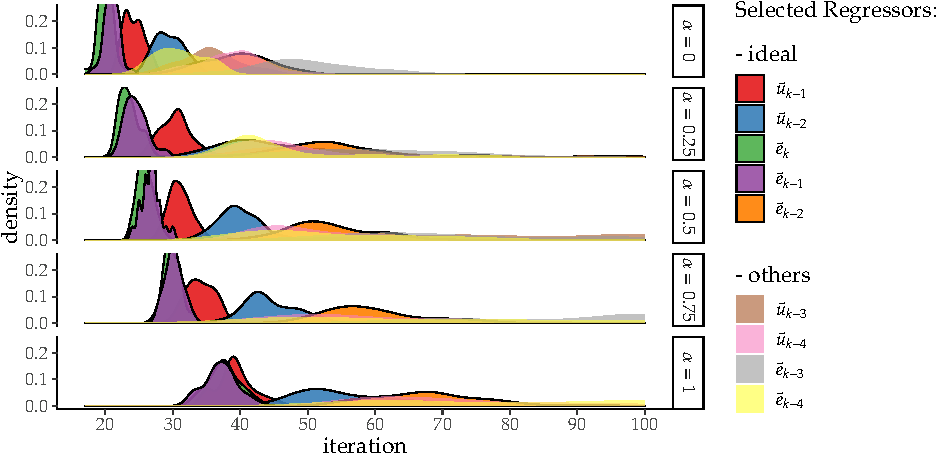
\includegraphics{Figs/Cap5/ex51_iter_con_COM_ruido.tex.pdf}
    \caption{Densidades de probabilidades para os regressores escolhidos para diferentes valores de $\alpha$, caso COM ruído.({\color{red} Caption ainda será mudada.})}
    \label{fig:exp51_itercon_ruido}
  \end{figure}



\end{exmp}


\begin{exmp}[RaCSS aplicado a um sistema não-linear] \label{ex:53}

  \todo[inline]{
    Neste exemplo a ideia é avaliar o comportamento do ``RaCSS'' a um sistema não-linear. Tomei um modelo de um aquecedor com dissipação variável adotado no seu livro. A ideia é apresentado o modelo no exemplo~\ref{ex:varHeater} da seção~\ref{sec:ramss}, no sentido do RaMSS para identificar o modelo. Depois aproveito o mesmo aqui para identificar o controlador.

    Por enquanto estão somente os gráficos, ainda falta análise e algumas tabelas comparativas com ERR.
  }



\end{exmp}
% =================================================================================================================

% \newpage
% \section{Rascunho}\label{sec:Rascunho}
%
%
% Como produto/trabalho em desenvolvimento durante o semestre, cita-se o trabalho que tem sido feito no sentido de desenvolver metodologias para escolha de estruturas para o controlador no âmbito do controle baseado em dados, ou DDC (Data-Driven Control).
% Mais especificamente, tem-se dado ênfase a escolha da estrutura do controlador a partir do uso de métodos VRFT.
% Como deixa claro em seu nome, ao usar o termo “sintonia” (em inglês, “tunning” ), a metodologia VR  FT visa a sintonia de um controlador pertencente a uma classe de controladores pré-estabelecida.
% Como abordado pelos autores do método~\citep{campi2002,campi2006a}, por outros estudiosos do assunto~\citep{bazanella2012} e apresentado neste relatório na seção de revisão bibliográfica, o método visa minimizar o erro de rastreamento de um modelo de referência pré-definido a partir da minimização de uma função de custo.
% Tal função é definida a partir do erro quadrático entre o sinal de excitação utilizado no processo a se controlar e o sinal de controle “virtual”, gerado pelo controlador identificado ao se aplicar  o mesmo sinal de referência capaz de produzir o mesmo sinal de saída  virtual utilizado na identificação.
%~\cite{campi2002} mostram, para o caso linear, e~\cite{campi2006}  e não linear, que ao se minimizar esta nova função de custos, minimiza-se também o erro de rastreamento, desde que se obedeça os seguintes critérios: a classe do controlador considerado tenha uma estrutura que possibilite abrigar o que se nomeia de controlador ideal (vide eq.
% ); que o processo não seja afetado por ruídos; e o controlador seja parametrizado linearmente.
% Caso o controlador ideal não possa ser representado pela classe considerada, o erro mínimo de rastreamento não é mais garantido e a introdução de um filtro ao projeto, visando se aproximar desse mínimo é desejado.
%
%
% No desenvolvimento do trabalho, foco deste relatório, tem-se feito um estudo de como seria possível, e quais as vantagens poderia-se obter se, ao invés de apenas tentar achar a melhor sintonia para um controlador com estrutura pré-estabelecida,  se procurasse também uma melhor estrutura dentro de um um conjunto de classes de controladores, de forma que o erro de rastreamento ótimo ou pelo menos sub-ótimo possa ser encontrado.
%
% Para atingir este propósito, tem-se investigado o uso de técnicas de seleção de estruturas que, com devidas adaptações e reformulações, sejam capazes selecionar modelos que resultem em controladores não lineares (ou mesmo lineares) que possam levar a respostas melhores do que aqueles que fazem uso de estruturas pré definidas.
%
% Dentre as ferramentas que têm-se utilizado, destacam-se o uso da taxa de redução de erro (ERR) e do algoritmo   Randomized Model Structure Selection (RaMSS)~\citep{falsone2014,falsone2015}. Estas estratégias têm sido estendidas e utilizadas em aplicações para determinação de modelos de processos dinâmicos~\citep{retesNARMAXModelIdentification2019} ou até mesmo no projeto de compensadores para aplicações em que o processo exibe determinados efeitos de não linearidade específicas, como no caso de efeitos histeréticos~\citep{abreuIdentificationNonlinearityCompensation2020}.

% Em particular, o método RaMSS, tem se mostrado promissor para a aplicação desejada. Esse método faz apelo às técnicas exploratórias que recorrem a buscas aleatórias ao estilo Monte Carlo, mas com mecanismos de seleção que reduzem drasticamente o custo computacional, evitando uma busca exaustiva, ao mesmo tempo em que tenta garantir uma seleção adequada.
%
% Apoiado nesta técnica, algumas adaptações têm sido estudadas no sentido de lidar agora com a identificação do controlador, e não mais do processo.
%
% Como abordado na revisão bibliográfica deste relatório, o método RaMSS faz uso de um índice de desempenho baseado no cálculo de alguma grandeza que quantifique a qualidade de o modelo em algum sentido. Uma escolha comum é calcular este índice baseado no erro quadrático médio de predição (MSPE).
%
% Um estudo sobre o uso deste índice tem sido feito na pesquisa em questão, conforme resultados apresentados na seção “Análise e Processamento de Dados”. O que se tem observado é que minimizar o MSPE diretamete pela estratégia RaMSS apesar de muitas vezes apresentar bons resultados, não dá garantias que o rastreamento ótimo é alcançado, i.e. aquele em que o erro de rastreamento médio quadrático por exemplo, é mínimo.
%
% Para sanar  esta deficiência, tem-se considerado o uso de algum índice que leve em conta o resultado final ao se aplicar os controladores intermediários identificados e selecionados pelo procedimento. Algo parecido tem sido usado no que diz respeito a identificação de processos  em que o erro quadrático médio de simulação (MSSE) é utilizado em substituição ao MSPE~\citep{aguirre2010}. Neste caso, segundo~\citep{piroddi2003}, o uso de informações da simulação-livre pode melhorar a robustez na seleção de estrutura do processo quando sob condições de identificabilidade parciais.
%
% O MSSE depende da simulação livre, que em suma é a resposta em malha aberta a um sinal de excitação conhecido. Algo parecido poderia ser utilizado ao se avaliar a estrutura no procedimento VRFT, porém, neste caso, seria desejável a resposta do sistema em malha fechada com o controlador obtido a partir da estrutura avaliada. O grande problema neste caso é que esta simulação passa a ser dependente de um modelo, ainda que aproximado do processo. Porém, como estratégias DDC visam exatamente não identificar um modelo para o processo, tal simulação torna-se inviável.
%
% No atual estágio desta pesquisa, tem-se trabalhado com a ideia de um índice que quantifique o erro médio de rastreamento em função do modelo do controlador sintonizado por uma estratégia VRFT, de modo que alguma informação da resposta em malha fechada com o controlador analisado possa ser usada para  o cálculo dos índices de probabilidades de inclusão do regressor, ou RIP (vide seção de Revisão Bibliográfica). Porém, como a simulação da resposta em malha fechada (ou mesmo malha aberta) é inviável devido a uma falta de modelo para o processo, o que se estuda é o uso de técnicas de Aprendizado por Reforço (RL) para que dados colhidos do processo real, enquanto em funcionamento, possam ser usados para o cálculo em tempo real dos RIP e consequentemente para  escolha de melhor estrutura.
%
% Algumas técnicas de RL se mostram promissoras neste caso, uma vez que muitas vezes levam à otimização de índices de desempenho a partir de dados amostrados, sem a necessidade do modelo do processo, ao mesmo tempo em que evitam o alto número de realizações amostrais como em metodologias Monte Carlo. Dentre elas a estratégia TD Learning, tem sido considerada, com uma atenção ao método conhecido como Q-learning, que permite que um controlador possa ser ajustado em uma abordagem conhecida como off-policy. Nesse caso, um controlador ou lei de controle (no caso do presente trabalho, mais precisamente sua estrutura) pode ser determinado enquanto o sistema em malha fechada obedece a uma lei (ou política) de controle diferente. Isto ajuda em eventuais problemas de instabilidade e exploração.
%
% Durante o semestre tem sido desenvolvido um algoritmo no intuito de implementar as ideiais consideradas anteriormente. Parte do algoritmo desenvolvido por Retes (2018), tem sido aproveitada, assim como algoritmos implementados e desenvolvidos pelo grupo do MACSIN1, grupo do qual o autor faz parte desde o início do doutorado. O algoritmo tem sido desenvolvido na linguagem R, portanto traduções de algumas ferramentas já disponíveis no MACSIN em outras linguagens tiveram e estão tendo que ser adaptadas. Os resultados apresentados na seção “Análise e Processamento de Dados” foram obtidos, em sua maioria, a partir deste algoritmo.

